\documentclass[11pt]{beamer}
\usepackage{verbatim}
\usepackage{amsmath}
\usepackage{amsthm}
\usepackage{graphics}
\usepackage{color}
\usepackage{stmaryrd}\usefonttheme[onlymath]{serif}

\title{On Multiphase-Linear Ranking Functions}
\date{\today}
\author{Xie Li}

\begin{document}
\maketitle

\begin{frame}\frametitle{Contributions}
\begin{itemize}
\item Equivalence of different classes of ranking function.

\item Algorithms for converting between ranking functions.

\item Converting ranking functions on integers to rational.

\item Depth bound and iteration bound for M$\Phi$RF.

\end{itemize}
\end{frame}

\begin{frame}\frametitle{Single Path Linear Constraint Loop}
\begin{example}
\begin{center}

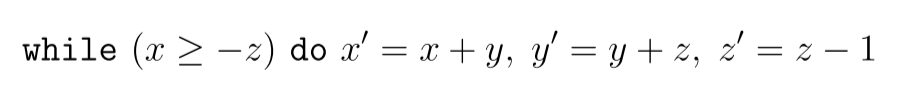
\includegraphics[scale = 0.4]{loopExample.png}

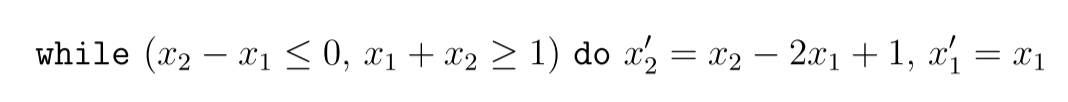
\includegraphics[scale = 0.4]{loopExample1.png}
\end{center}

\end{example}

\begin{definition}[SLC]
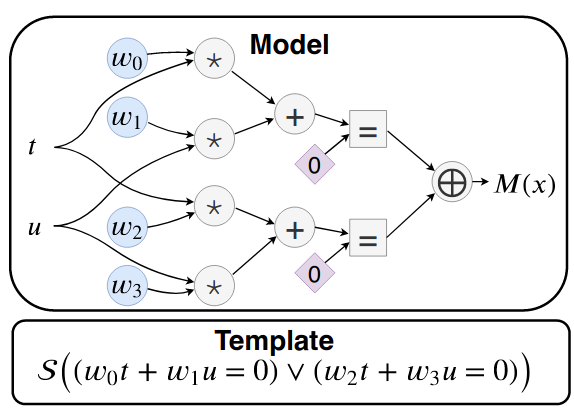
\includegraphics[scale = 0.4]{1.png}


\end{definition}
\begin{center}
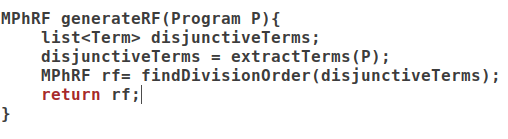
\includegraphics[scale = 0.35]{2.png}

$A''\textbf{x}'' \le \textbf{c}''$
\end{center}


\end{frame}

\begin{frame}\frametitle{Ranking Functions}

\begin{definition}[Linear Ranking Function(LRF)]

$f(x_1, \ldots, x_n) = a_1x_1 + \ldots a_nx_n + a_0$, such that

\begin{itemize}
\item $f(\textbf{x}) \ge 0$ for any $\textbf{x}$ satisfies the loop constraints.

\item $f(\textbf{x}) - f(\textbf{x}') \ge 1$ for any transition from $\textbf{x}$ to $\textbf{x}'$.



\end{itemize}
\end{definition}

\begin{example}
\[\texttt{while }( x - 1 > 0) \texttt{do } x' = x - 5\]

Its LRF: $f(x) = x - 1$
\end{example}

We can define a binary relation $\textbf{x} \succeq \textbf{x}'$ iff  $f(\textbf{x}) - f(\textbf{x}') \ge 1$ and $f(\textbf{x}) \ge 0$

\end{frame}


\begin{frame}\frametitle{Example: Nested Ranking Function}


\end{frame}

\begin{frame}\frametitle{Example: Multiphase Ranking Function}
Problem: LRF is not strong enough for all loops.
\begin{example}
\[\texttt{while }( x > -z) \texttt{do } x' = x + y, y' = y + z, z = z - 1\]

$f(x, y, z) = a_1x + a_2y + a_3z + b$

assume $a_1, a_2, a_3$ and $b$ are given, 

\[f(x, y, z) - f(x', y', z') = a_3 + ya_1 + za_2\]

variable $y, z$ do not have bound and cannot be used in the ranking function.
\end{example}

\end{frame}


\begin{frame}\frametitle{Example: Multiphase Ranking Function}
\[\texttt{while }( x > -z) \texttt{do } x' = x + y, y' = y + z, z = z - 1\]

Attempt to use a ranking function that has several phases: 
$\langle z + 1, y + 1, x\rangle$
\begin{center}
\begin{tabular}{|c|c|c|c|c|c|}
\hline 
$x$&$y$&$z$&$z+1$&$y+1$&$x$\\
\hline
$1$&$1$&$1$&\textbf{2}&$2$&$1$\\
$2$&$2$&$0$&\textbf{1}&$3$&$2$\\
$4$&$2$&$-1$&\textbf{0}&$3$&$4$\\
\hline
$6$&$1$&$-2$&$-1$&\textbf{2}&$6$\\
$7$&$-1$&$-3$&$-2$&\textbf{0}&$7$\\
\hline
$6$&$-4$&$-4$&$-3$&$-3$&\textbf{6}\\
$2$&$-8$&$-5$&$-4$&$-7$&\textbf{2}\\
\hline
$-6$&$-13$&$-6$&$-5$&$-12$&$-6$\\
\hline
\end{tabular}
\end{center}
\end{frame}



\begin{frame}{Multiphase Ranking Function}
\begin{definition}
Given a set of transitions $T\subseteq \mathbb{Q}^{2n}$, we say $\langle f_1, \ldots, f_d\rangle$ is a multiphase ranking function for $T$ if for every $\textbf{x}'' \in T$, there is an index $i\in [1, d]$, s.t.

\begin{center}
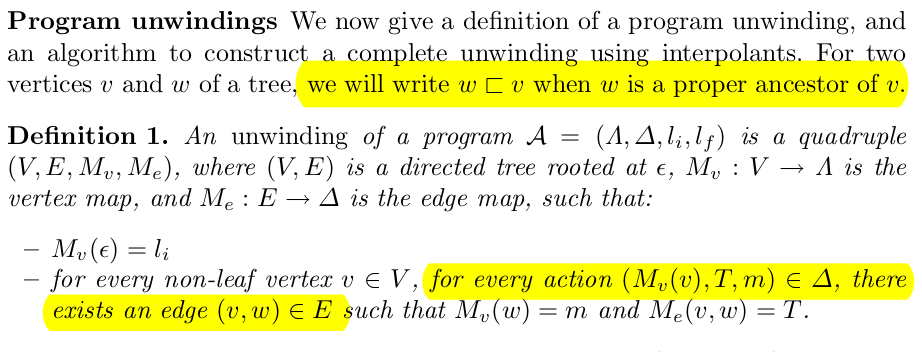
\includegraphics[scale = 0.3]{3.png}
\end{center}
We say that $\textbf{x}''$ is ranked by $f_i$(for the minimal).
\end{definition}


\end{frame}


\begin{frame}\frametitle{Example Revisit}
\[\texttt{while }( x > -z) \texttt{do } x' = x + y, y' = y + z, z = z - 1\]

\begin{center}
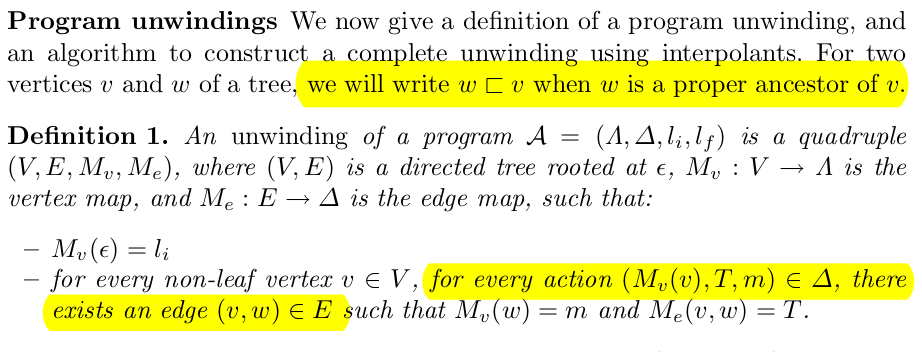
\includegraphics[scale = 0.2]{3.png}

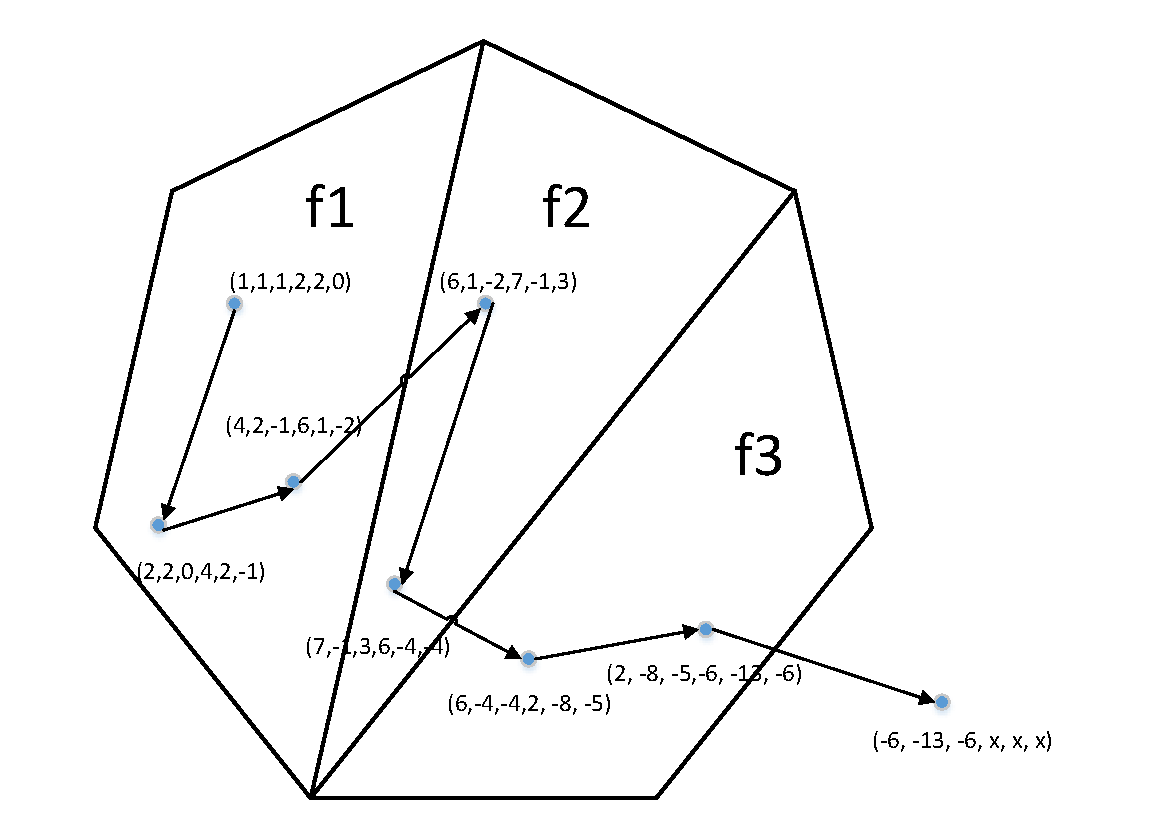
\includegraphics[scale = 0.4]{3.pdf}
\end{center}
\end{frame}


\begin{frame}\frametitle{Nested Ranking Function}
\[\texttt{while }( x > -z) \texttt{do } x' = x + y, y' = y + z, z = z - 1\]

Loop condition: $x + z > 0$. We only want to use this constraint for the ranking function.

$\langle z + 1, y + 1, x + z\rangle$


\begin{definition}[Nested Ranking Function]

A tuple $\langle f_1, \ldots, f_d\rangle$ is a nested ranking function for $T$ if the following requirements are satisfied for all $\textbf{x}''\in T$
\begin{center}
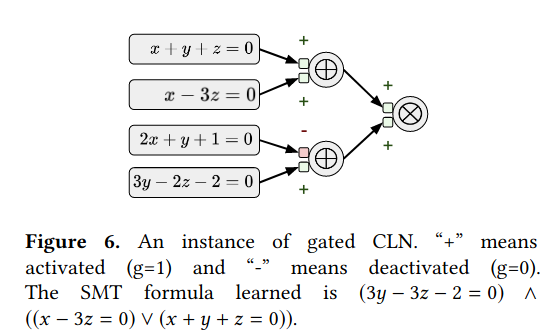
\includegraphics[scale = 0.3]{6.png}

\end{center}

Let $f_0 = 0$.
\end{definition}

Nested is Multiphase, but not the opposite.

($x = -1, y = 0 , z = 1$)
\end{frame}

\begin{frame}{M$\Phi$RF to Nested Ranking Function?}
\begin{theorem}
If $T$ has a M$\Phi$RF of depth $d$, then it has a nested ranking function of depth at most $d$. 

\end{theorem}

Sythesising nested ranking function is in \texttt{PTIME}, with theorem above we have..
\end{frame}

\begin{frame}\frametitle{Lexicography Linear Ranking Function}

Intuition: remind binary relation $\textbf{x} \succeq \textbf{x}'$ iff  $f(\textbf{x}) - f(\textbf{x}') \ge 1$ and $f(\textbf{x}) \ge 0$.

Generalize it into several phases using lexicographical order of ranking functions.

$\langle f_1, f_2, \ldots, f_d\rangle$

$(2,3,1,3) \ge (2,1,5,4)$

\begin{definition}[LLRF]
Given a set of transitions $T$ we say that 
$\langle f_1, f_2, \ldots, f_d\rangle$ is a LLRF (of depth $d$) for $T$ if for every $\textbf{x}''\in T$ there is an index $i$ such that 
\begin{center}
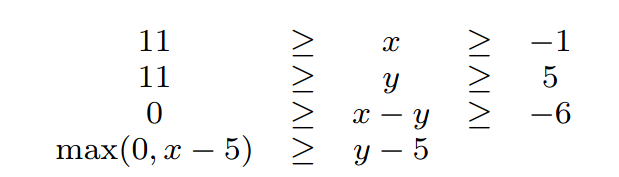
\includegraphics[scale = 0.26]{4.png}

\end{center}
A LLRF is weak if..
\end{definition}
\end{frame}



\begin{frame}\frametitle{Example: M$\Phi$RF is a LLRF}
\begin{center}
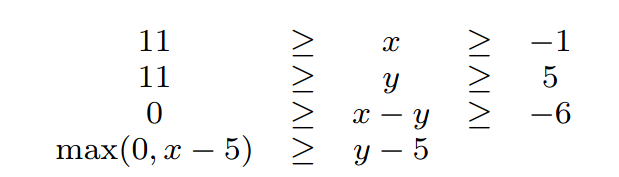
\includegraphics[scale = 0.2]{4.png}
\end{center}
\[\texttt{while }( x > -z) \texttt{do } x' = x + y, y' = y + z, z = z - 1\]

\begin{center}
\begin{tabular}{|c|c|c|c|c|c|}
\hline 
$x$&$y$&$z$&$z+1$&$y+1$&$x$\\
\hline
$1$&$1$&$1$&$2$&$2$&$1$\\
$2$&$2$&$0$&$1$&$3$&$2$\\
$4$&$2$&$-1$&$0$&$3$&$4$\\
\hline
$6$&$1$&$-2$&$-1$&$2$&$6$\\
$7$&$-1$&$-3$&$-2$&$0$&$7$\\
\hline
$6$&$-4$&$-4$&$-3$&$-3$&$6$\\
$2$&$-8$&$-5$&$-4$&$-7$&$2$\\
\hline
$-6$&$-13$&$-6$&$-5$&$-12$&$-6$\\
\hline
\end{tabular}
\end{center}

\end{frame}

\begin{frame}{LLRF to M$\Phi$RF?}
\begin{theorem}[weak LLRF to M$\Phi$RF]
If $T$ has a weak $LLRF$ of depth $d$, it has a M$\Phi$RF of depth $d$.

\end{theorem}

\end{frame}

\begin{frame}\frametitle{Ranking Function Over Integers}\
\[A''\textbf{x}''\le \textbf{c}\]

\begin{itemize}
\item Rational convex polyhedra: polyhedra defined by $\mathcal{P}=\{\textbf{x}''\in \mathbb{Q}^{2n}\mid A''\textbf{x}''\le \textbf{c}\}$.

\item Integers: $I(\mathcal{P}) = \mathcal{P} \cap \mathbb{Z}^{2n}$

\item Integer hull: $\mathcal{Q}_I$ is the space of convex combinition of points in $I(\mathcal{P})$.

\end{itemize}

\end{frame}

\begin{frame}\frametitle{Why consider integer?}
\begin{itemize}
\item Actual programs with \texttt{int}.

\item More important, conclusions for rational does not always applicable in on integer version.

\end{itemize}
\begin{example}
\begin{center}

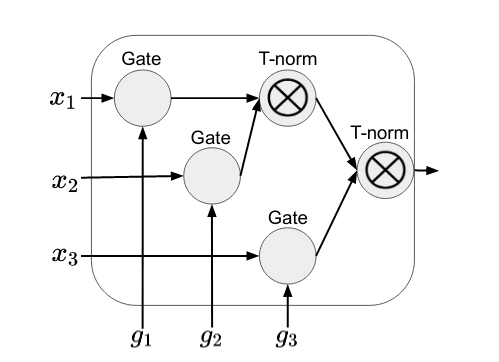
\includegraphics[scale = .3]{7.png}

\end{center}
For rationals: $x_1 = \dfrac{1}{2}, x_2 = \dfrac{1}{2}$

For integers: there exists a linear ranking function $f(x_1, x_2) = x_1 + x_2$
\end{example}
\end{frame}

\begin{frame}\frametitle{Integer to Rational}
\begin{theorem}
Let $\langle f_1, f_2, \ldots, f_d\rangle$ be a weak LLRF for $I(\mathcal{P})$. Then there are constants $c_1, \ldots, c_d$ such that $\langle f_1 + c_1, f_2 + c_2, \ldots, f_d + c_d\rangle$ is a weak LLRF for $\mathcal{Q}_I$

\end{theorem}
\end{frame}

\begin{frame}\frametitle{The Depth of a M$\Phi$RF}
Idea:  precompute an upper bound of depth $\rightarrow$ a decision procedure for M$\Phi$RF in general


\begin{theorem}
For integer $B > 0$, following loop needs at lease $B+1$ components in any M$\Phi$RF.
\begin{center}
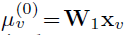
\includegraphics[scale = 0.4]{5.png}

\end{center}
\begin{example}

\begin{center}
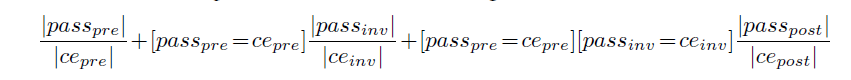
\includegraphics[scale = 0.4]{8.png}

\end{center}
\end{example}
\end{theorem}
\end{frame}


\begin{frame}\frametitle{Iteration Bound}
\begin{theorem}

An SLC loop that has a M$\Phi$RF terminates in a number of iterations bounded by $O(||x_0||_{\infty})$
\end{theorem}

\end{frame}

\begin{frame}
\begin{center}
\textbf{Future Work \& Questions}
\end{center}
\end{frame}
\end{document}